\documentclass[fontsize=12pt]{article}

\usepackage{listings}
\usepackage[T1,T2A]{fontenc}
\usepackage[utf8]{inputenc}
\usepackage[russian]{babel}
\usepackage{amsmath}
\usepackage{xcolor}
\usepackage{scrextend}
\usepackage{enumerate}
\usepackage{graphicx}
\usepackage{minted}
\usepackage[left=1.5cm,right=1.5cm,top=1.5cm,bottom=1.5cm,bindingoffset=0cm]{geometry}


\linespread{1.3}
\parindent=0.6cm
\lstset{tabsize = 2}
\graphicspath{ {./images/} }

\title{Курсовая работа}
\author{Лев Довжик, M3439}
\date{}


\begin{document}
	\pagenumbering{gobble}
	\maketitle
	
\section{ERM}

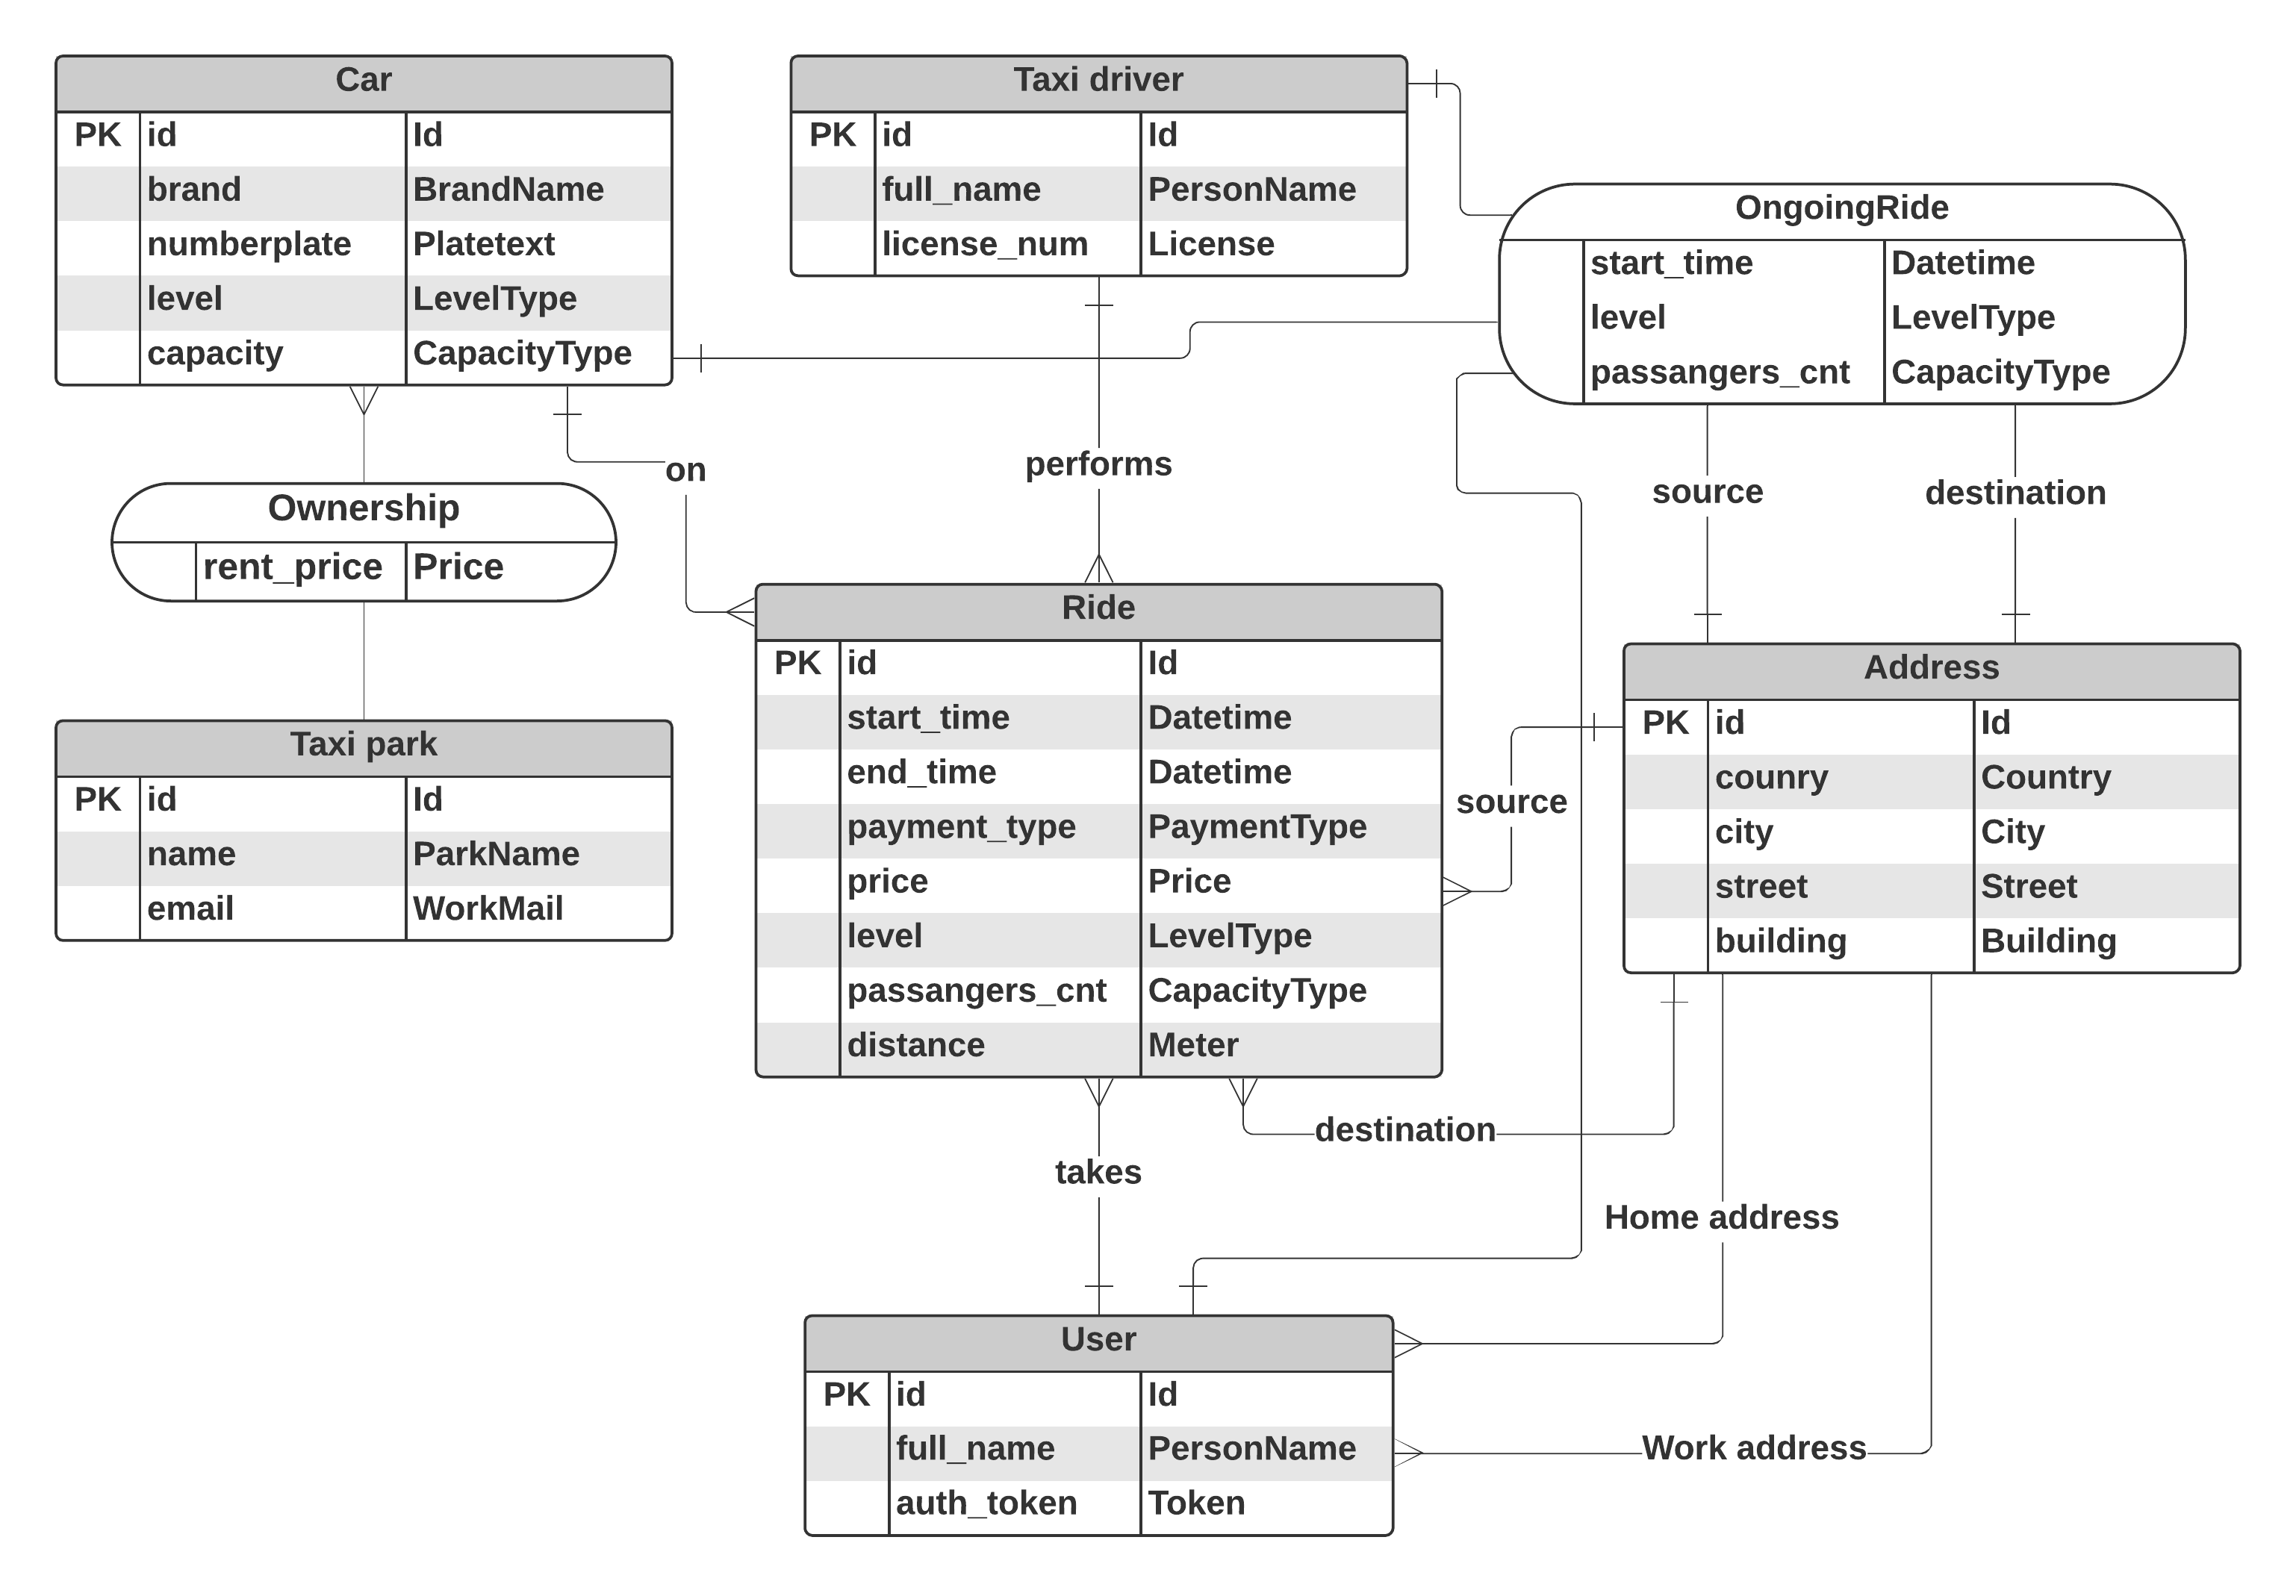
\includegraphics[scale=0.72]{Taxi.png}

Каждый пользователь, каждая машина и каждый водитель может состоять не более чем в одной ассоциации $OngoingRides$, при в ней всегда определены все три эти элемента. Также при фиксированных остальных членах может быть лишь один $source$ и один $destination$.

\section{Физическая модель}

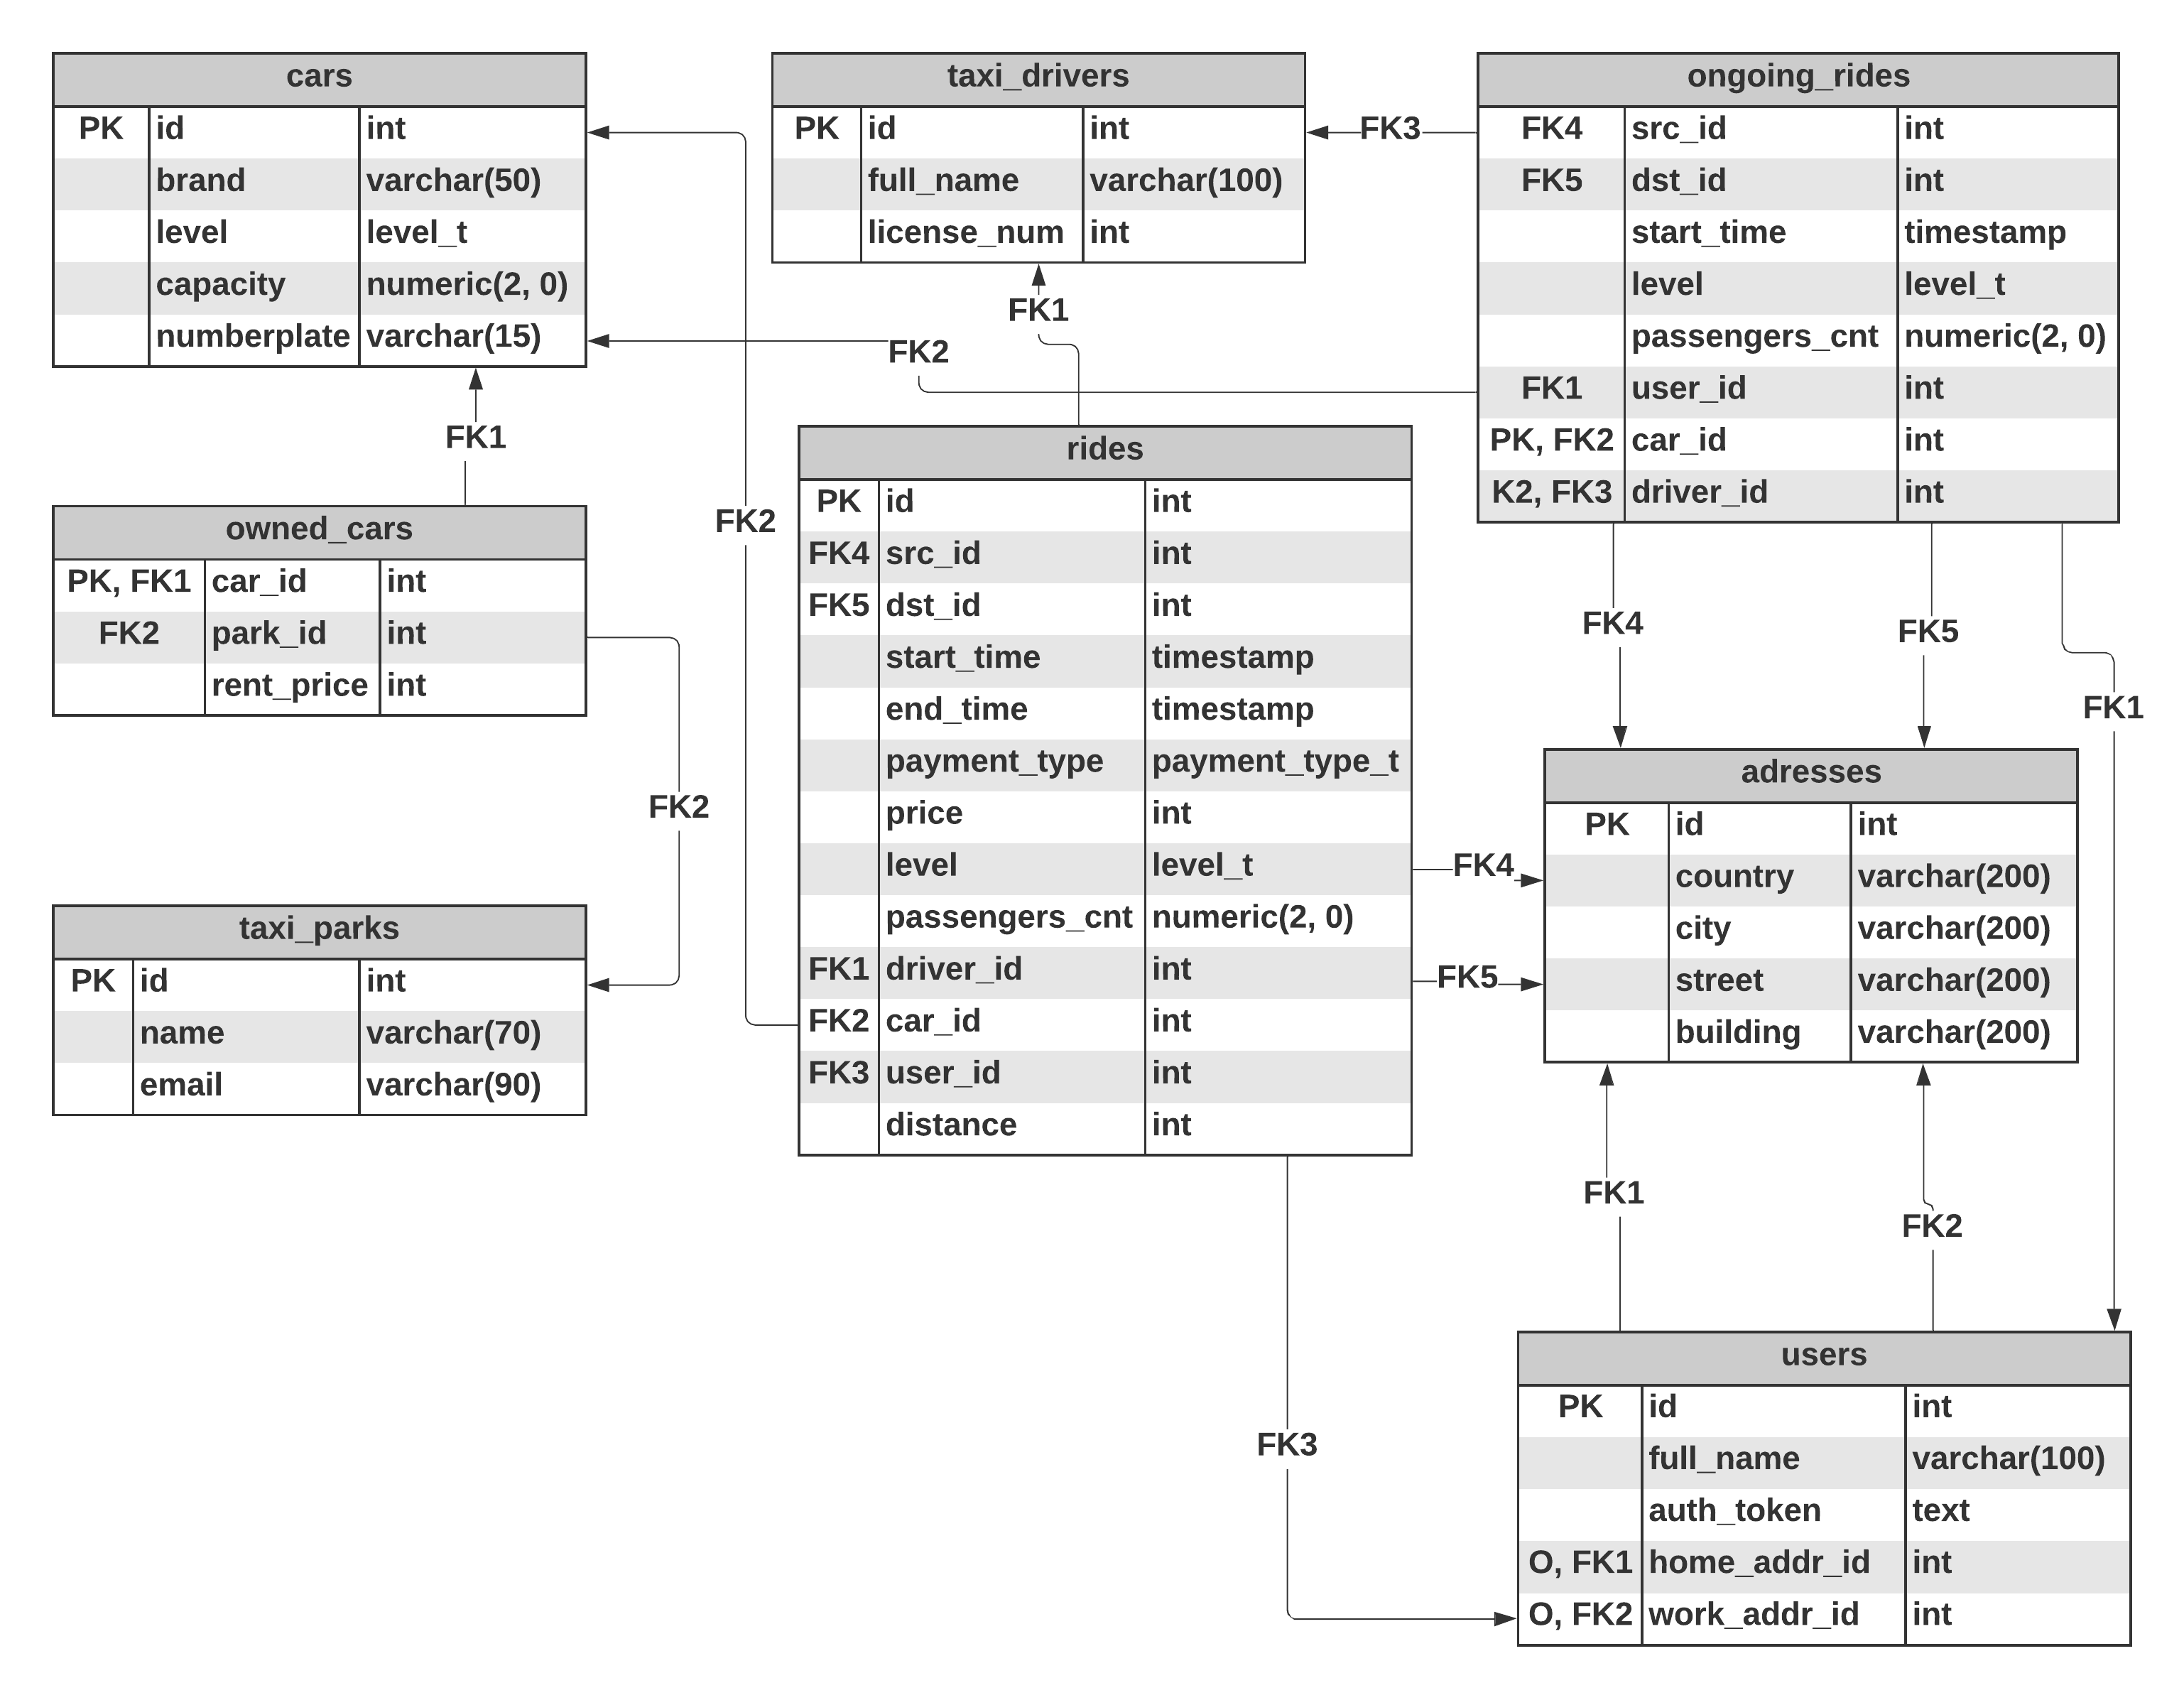
\includegraphics[scale=0.7]{Taxi_phys.png}

\section{Функциональные зависимости}

\subsection{cars}

В данном отношении имеются 4 нетривиальные ФЗ: $id \rightarrow brand$, $id \rightarrow level$, $id \rightarrow capacity$, $id \rightarrow numberplate$. Остальные ФЗ получаются из данных и тривиальных по правилам вывода. 

В связи с тем, что замыкание $id$ с данным ФЗ и самоопределением даёт все атрибуты, а само множество неприводимо, то оно эквивалентно всем ФЗ данного отношения, a $id$ является ключом.

\subsection{owned\_cars}

В данном отношении имеются 2 нетривиальные ФЗ: $car\_id \rightarrow park\_id$, $car\_id \rightarrow rent\_price$. Остальные ФЗ получаются из данных и тривиальных по правилам вывода. 

В связи с тем, что замыкание $car\_id$ с данным ФЗ и самоопределением даёт все атрибуты, а само множество неприводимо, то оно эквивалентно всем ФЗ данного отношения, a $car\_id$ является ключом.

\subsection{users}

В данном отношении имеются 1 нетривиальная ФЗ: $id \rightarrow full\_name, id \rightarrow auth\_token, id \rightarrow home\_addr\_id, id \rightarrow work\_addr\_id$. Остальные ФЗ получаются из данной и тривиальных по правилам вывода. 

В связи с тем, что замыкание $id$ с данным ФЗ и самоопределением даёт все атрибуты, а само множество неприводимо, то оно эквивалентно всем ФЗ данного отношения, a $id$ является ключом.

\subsection{taxi\_drivers}

В данном отношении имеются 2 нетривиальные ФЗ: $id \rightarrow full\_name$, $id \rightarrow licens\_num$. Остальные ФЗ получаются из данных и тривиальных по правилам вывода. 

В связи с тем, что замыкание $id$ с данным ФЗ и самоопределением даёт все атрибуты, а само множество неприводимо, то оно эквивалентно всем ФЗ данного отношения, a $id$ является ключом.

\subsection{addresses}

В данном отношении имеются 1 нетривиальная ФЗ: $id \rightarrow name$. Остальные ФЗ получаются из данной и тривиальных по правилам вывода. 

В связи с тем, что замыкание $id$ с данным ФЗ и самоопределением даёт все атрибуты, а само множество неприводимо, то оно эквивалентно всем ФЗ данного отношения, a $id$ является ключом.

\subsection{rides}

В данном отношении все нетривиальные ФЗ имеют вид $id \rightarrow ?$. Остальные ФЗ получаются из данных и тривиальных по правилам вывода. 

В связи с тем, что замыкание $id$ с данным ФЗ и самоопределением даёт все атрибуты, а само множество неприводимо, то оно эквивалентно всем ФЗ данного отношения, a $id$ является ключом.

\subsection{ongoning\_rides}

В данном отношении, во первых все атрибуты функционально зависят от $user\_id$, значит замыкание его с самоопределением  даёт все атрибуты, а самом он является ключом. Однако так же в тройке $user\_id, car\_id$ и $driver\_id$ любой из атрибутов однозначно определяет остальные два. В таком случае каждый из них является ключём. 

\section{Нормализация}

\subsection*{1 нормальная форма}

Во всех наших отношениях нет повторяющихся групп, все атрибуты атомарны и присутствует ключ, значит, все они находятся в 1 н.ф.

\subsection*{2 нормальная форма}

Все отношения в 1 н.ф., а так же выше было показано, что все неключевые атрибуты зависят от целого ключа, значит, все они в 2 н.ф.

\subsection*{3 нормальная форма}

Все отношения во 2 н.ф., а так же было показано выше, что все неключевые атрибуты напрямую зависят от ключей, значит все они в 3 н.ф.

\subsection*{Нормальная форма Бойса-Кодда}

Заметим, что во всех наших отношениях все нетривиальны функциональные зависимости имели вид $\left< soeme\_id \right> \rightarrow ?$ или же выводились с их участием. Следовательно их левая часть является надмножеством ключа, т.е. надключом. Отсюда делаем вывод, что все отношения находятся в НФБК.

\subsection*{4 нормальная форма}

В каждом из этих отношений есть простой ключ($\left< soeme\_id \right>$) и они находятся в НФБК, следовательно, по 2 теореме Дейта-Фейгина они находятся в 4 н.ф.

\subsection*{5 нормальная форма}

В всех отношениях все ключи имеют вид $\left< soeme\_id \right>$ т.е является простыми. Во всех отношениях, кроме $ongoing_calls$ все нетривиальные ФЗ содержат его лишь в левой части, значит замыкание остальных атрибутов не будет содержать $id$. Следовательно он является частью любого ключа, а так как он сам по себе ключ, то он является единственным ключом причём простым. В $ongoing_calls$ так же логика верна, если убрать три известных простых ключа, т.е. они являются единственными ключами.

В таком случае, в силу того, что все эти отношения находятся в 3 н.ф., по первой теореме Дейта-Фейгина, они так же находятся в 5 н.ф.

\section{База данных в PostgeSQL}

\subsection{Объявление}

\inputminted[frame=single]{sql}{scripts/create-database.sql}

\subsection{Ограничения}

\inputminted[frame=single]{sql}{scripts/add-constraints.sql}

\subsection{Индексы}

PostgreSQL создаёт древесные индексы для всех \textbf{PRIMARY KEY} и \textbf{UNIQUE}, а так же для всех \textbf{EXCLUDE} ограничений с помощью $gist$. Добавим же ещё несколько индексов для ускорения запросов:

\inputminted[frame=single]{sql}{scripts/add-indexes.sql}

\section{Заполнение БД}

Так как существующие агрегаторы не делятся данным о поездках и пользователях, заполним таблицу случайными данными

\inputminted[frame=single, fontsize=\small]{python}{scripts/fill-database.py}
	
При запуске скрипта не удалось всего 82 вставки поездок.	

\section{Функции для работы и запросы}

\subsection*{Добавление пользователя}

Наша база данных хранит пароли в зашифрованном виде, для удобства работы вся работа по их шифрованию лежит на плечах это базы, которая и предоставляет API:

\inputminted[frame=single]{sql}{scripts/functions/add-user.sql}

\subsection*{Изменение пользовательских адресов}

У пользователя есть возможность сохранить в быстрый доступ домашний и рабочий адрес, однако кто попало не может их изменять, для этого есть специальные функции производящие все проверки:

\inputminted[frame=single]{sql}{scripts/functions/modify-user-address.sql}

\subsection*{Средняя скорость}

Одной из полезных характеристик водителя является скорость его вождения. Кому-то из пользователей нравятся спокойные поездки по городу, другим же интересно как можно быстрее добраться из точки А в точку Б. Заведём же \textbf{view} для этой характеристики:

\inputminted[frame=single]{sql}{scripts/views/average-speed.sql}

\subsection*{Количество апгрейдов за период}

На заказ с определённым уровнем комфорта может откликнуться любая машина с большим либо равным уровнем. Однако для такси это является неоптимальным расходованием ресурсов. Хочется уметь получать эту информацию, чтобы правильно оценивать количество машин каждого класса, которые нам нужны сейчас на линии, для этого заведём \textbf{view} со всеми апгрейдами, из которого будет получать статистику за нужный период:

\inputminted[frame=single]{sql}{scripts/views/upgrades.sql}

\inputminted[frame=single]{sql}{scripts/functions/upgrades-in-period.sql}

\subsection*{Распределение способов оплаты}

Полезно знать, как часто чем пользуется пользователи, что проводить акции с партнёрами или улучшать соответствующую инфраструктур:

\inputminted[frame=single]{sql}{scripts/queries/payment-type-distribution.sql}

\subsection*{Статистика за год}

Многие сервисы подводят какую-то статистику по пользователям за год, а потом показывают её им. Мы не являемся исключением:

\inputminted[frame=single]{sql}{scripts/functions/user-year-statistics.sql}

\subsection*{Распределение заказов по времени}

Количество заказов разнится в течении дня, знание этого распределения помогут правильно выставлять машину на линию:

\inputminted[frame=single]{sql}{scripts/functions/rides-hour-distribution.sql}

\subsection*{Валидация пользователей}

Запрос, который пригодится при любых запросах от пользователей для проверки их входных данных:

\inputminted[frame=single]{sql}{scripts/functions/validate-user.sql}

\subsection*{Завершение поездки}

В такси водитель заканчивает поездку, сделаем же удобную функцию которая позволяет это сделать, добавив необходимую информацию в соответствующую таблицу:

\inputminted[frame=single]{sql}{scripts/functions/finish-ride.sql}

\section{Уровни изоляции запросов}

\subsection*{Добавление пользователя}

В данном запросы мы читаем всего один раз не более чем одну строку, а затем пишем. В таком случае нам достаточно \textbf{read commited} уровня изоляции. От фантомных же записей нас сохраняют ограничение $PRIMARY\ KEY$ на $taxi\_users.id$.


\subsection*{Изменение пользовательских адресов}

В данных запросах мы так же читаем 1 раз 1 строку, в потом в неё пишем. Фантомные записи на не страшны так как мы не производим никаких вставок, и не ориентируемся на другие строки таблицы. Исходя из этого \textbf{read commited} будет достаточно.

\subsection*{Средняя скорость}

Это большой но read-only запрос, однако результаты его вряд ли сильно меняются за время его исполнения. К тому же в таблице $taxi_drivers$ вряд ли происходит много изменений, а в таблице $rides$ подавляющие число изменений append-only, что так же исходя из вышесказанного не сильно искажает результат.

Исходя из всего этого можно заключить, что \textbf{read uncommited} будет вполне достаточно. 

\subsection*{Количество апгрейдов за период}

Тяжесть этого запроса зависит от размера периода и проходится он по таблице в преимущественно append-only изменениями. В таком случае главной нашей проблемой могут быть фантомные записи, если конец периода близок к текущему времени. Однако за большой такой период такие записи вряд ли внесут серьёзные изменения, а за маленький запроса отработает достаточно быстро, что так же уменьшит погрешность. От фантомных записей ничего кроме \textbf{serializable} не спасает, а тормозит работу мы не хотим. В таком случае можно выбрать самый дешёвый из оставшихся уровней: \textbf{read uncommited}.

\subsection*{Распределение способов оплаты}

Тяжесть этого запроса зависит от периода, который мы запрашиваем. Сам запрос read-only, и пробегается по таблице, в которой подавляющие число изменений append-only. Однако вряд ли данные за очень короткий период в настоящем будут в любом случае сколько-то репрезентативны Исходя из этого \textbf{read uncommited} уровня изоляции ему должно хватить.

\subsection*{Статистика за год}

Данные для этого запроса почти не меняются так как собираются за целый год, но в связи с этим объём их велик и не хочется чтобы он блокировал работу сервиса под Новый Год (скорее всего в это время его будут запускать). В таком случае снова \textbf{read uncommited}.

\subsection*{Распределение заказов по времени}

Логика ограничений этого запроса полностью аналогична запросу распределения способов оплаты, так что \textbf{read uncommited}.

\subsection*{Валидация пользователей}

Несмотря на то что этот запрос read-only и читает всего одну строку из таблицы, логика его использования подразумевает, чтобы данные были корректны в какой-то момент времени для линеризации транзакций. Исходя из этого выбираем \textbf{read commited}.

\subsection*{Завершение поездки}

В силу того, что мы читаем из таблицы $ongoing\_rides$ один раз, фантомные вставки в неё нам не страшны, подобные же вставки в $rides$ будет отловлены ограничениями $PRIMARY\ KEY$. В таком случае нам достаточно \textbf{read commited}.

\section{Пример работы}

В данном примере мы начинаем и заканчиваем поездку, а затем смотрим статистику по пользователям в 2020 году(в будущем эти даты стоит поменять).

\inputminted[frame=single]{sql}{scripts/examples.sql}

\end{document}

